%!TEX TS-program = xelatex
%!TEX encoding = UTF-8 Unicode
\documentclass{ctexart}
\usepackage[a4paper,hmargin=0.7in,vmargin=0.75in]{geometry}
\usepackage{setspace}
\usepackage{listings}
\linespread{1.5}
\newfontfamily\listingsfont{Menlo}
\lstset{breaklines,frame=single,basicstyle=\linespread{0.6}}
\usepackage[nounderscore]{syntax}
\setlength{\parskip}{1em}
\newenvironment{typewriterfont}{\ttfamily}{\par}

\title{从MiniC到RiscV \\ \large 编译实习课程报告}
\author{1500012739 特古斯}

\begin{document}
\maketitle{}
\tableofcontents
\newpage

\section{综述}

这学期的编译实习的任务是从MiniC(简化版的C)$\rightarrow$中间代码Eeyore$\rightarrow$中间代码Tigger$\rightarrow$RiscV伪汇编,每个阶段都有一定的检查以确保此阶段的正确性和进度的进展。从零开始做一个编译器的确是非常有成就感的一件事,我也在其中很大的提升了自己的代码能力。

这学期的编译实习与以往不同,第一次采用MiniC作为课程的语言平台。相对于原来的MiniJava,MiniC的语法更加简单,剔除了面向对象的内容,简化了许多的工作。但与此同时,课程设计者在课程设计也中有些缺陷和考虑欠妥的地方,经过今年的实践,我也对课程有一些建设性的提议。

\section{实验平台}

在整个实现过程中我全部采用了Lex+Yacc工具链进行翻译,因为翻译过程遵循同样的模式,修改起来也比较方便。我也曾经尝试过用Python用正则表达式匹配进行中间代码优化,不过后来由于过于繁琐还是直接用Yacc生成的代码优化了。

Yacc是一个采用LALR(1)语法分析的工具,输入BNF并添加语义规则就可以生成需要的代码,一般都要与Lex结合。Lex则是一个用正则表达式分析语言,把每个符号分解为Token进一步输入Yacc。

下面是对每个部分方法详述。

\section{MiniC}

这部分的任务是分析MiniC的语法并翻译成Eeyore。MiniC的语法比C简单了许多,不过原来的文档提供的BNF有许多漏洞,我也在基础之上加上了许多的小优化,下面是我实现的BNF。
\subsection{BNF}
\setlength{\grammarindent}{8em} % increase separation between LHS/RHS
\begin{typewriterfont}
\begin{grammar}
<Goal> ::= DefnDeclList*

<DefnDeclList> ::= (VarDefn|FuncDefn|FuncDecl)*

<VarDefn> ::= Type Identifier ';'
\alt Type Identifier '['<INTEGER>']' ';'
\alt Type Identifier '=' Expression ';' //声明时赋值
\alt Type Identifier '['<INTEGER>']' '=' Expression ';'

<VarDecl> ::= Type Identifier
\alt Type Identifier'['<INTEGER>?']'

<FuncDefn>  ::= Type Identifier '(' ( VarDecl ( ',' VarDecl )* )? ')' '\{' (FuncDecl | Statement)* '\}'

<FuncDecl> ::= Type Identifier '(' ( VarDecl (',' VarDecl)*)?')' ';'

% <MainFunc> ::= 'int' 'main' '(' ')' '\{' (FuncDecl | Statement)* '\}'

<Type> ::= 'int'

<Statement> ::= '\{' (Statement)* '\}'
\alt 'if' '(' Expression ')' Statement ('else' Statement)?
\alt 'while' '(' Expression ')' Statement
\alt Identifier '=' Expression ';'
\alt Identifier '[' Expression ']' '=' Expression ';'
\alt Expression // 无左值表达式
\alt 'return' Expression ';'

<Expression>	::=	Expression ( '+' | '-' | '*' | '/' | '\%' ) Expression
\alt Expression ( '\&\&' | '||' | '\textless' | '==' | '\textgreater' | '!=' ) Expression
\alt Expression '[' Expression ']'
\alt <INTEGER>
\alt Identifier
\alt ( '!' | '-' ) Expression
\alt Identifier '(' (Expression (',' Expression)*)? ')' // 参数支持表达式
\alt '(' Expression ')'

<Identifier>	::=	<IDENTIFIER>

\end{grammar}
\end{typewriterfont}

\subsection{特点}

\begin{itemize}
  \item \textbf{增加了对新语法的支持}

  与原来的BNF比较,增加了
  \begin{itemize}
    \item 无返回值表达式,如直接调用函数
    \item 表达式传入任何可传入的位置(如函数参数)
    \item 声明时直接赋值
  \end{itemize}

  同时支持在函数中声明与定义函数,作用域为最近的域。

  \item \textbf{对代码进行检查}
  \begin{itemize}
    \item 未声明变量或函数
    直接报错,输出出错行数并停止翻译
    \item 重复定义变量
    采用第一次定义的变量
    \item 函数参数数量不匹配
    直接报错,输出出错行数
    \item 语法错误
    直接报错,输出出错行数
  \end{itemize}

\end{itemize}

\subsection{实现细节}

\begin{lstlisting}[basicstyle=\listingsfont,caption={环境结构},captionpos=b]
typedef struct environment
  {
    struct environment* pre;//前向指针
    map<string,string> symTable;//符号表
    map<string,string> declList;//已声明函数
    map<string,string> funcPara;//函数参数
    int varCnt;
  } Env;
\end{lstlisting}

整个过程使用了On-the-fly动态生成的方法,同时考虑到并不需要特别多的依赖关系,每个非终结符号都可以用string代表它所代表的变量,整个过程非常的简洁。因为这个原因,符号表中只需存储MiniC中每个变量名和对应的eeyore临时变量名,用一个map表示符号表即可。而不同的环境用一个链表串起来,在每个环境中存储的信息只有符号表、已声明的变量集合(用来判断是否有未声明的变量)和函数参数。

\begin{figure}[htbp]
  \centering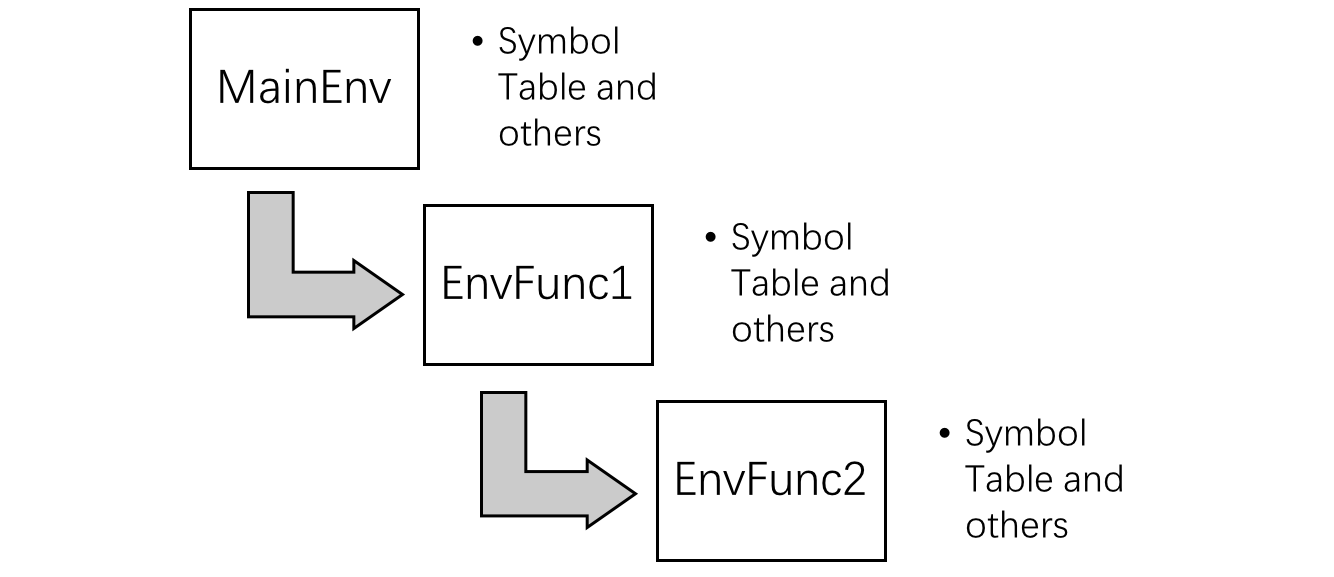
\includegraphics[width=8cm]{latexIMG/MiniCEnv.png}
  \caption{环境示意图}
  \label{}
\end{figure}

\subsection{编写中遇到的问题}

首先是没有理解Eeyore中变量的命名方式,一开始直接用T开头后面加乱七八糟的字母来方便调试,结果一直跑不通…才发现后面必须是标准的数字。

还有就是两方符号的识别与命名:每次识别到新的符号,直接把所有符号先转换为内部的独有变量,不过这样也带来了一些问题:对Identifier来说没有上下文信息,不好判断是在什么地方进行的,因此需要全局变量来辅助,这样也造成了一些结构上比较丑陋的地方,不过总体来说利大于弊。

为了翻译上的方便,我一开始使用了大量的临时变量存储中间结果,这也给后来的优化埋下了很多伏笔。

\subsection{实现过程中的小Tips}

因为On-the-fly生成时不存在显式的语法树,有些必须的辅助信息(如判断是否为函数参数)需要作为继承属性输入到下层的非终结符号中,而我把每个符号的类型都设置成了string……因此我就用了各种方法对栈中进行传递,比如全局变量和临时的环境。

总体来看,在MiniC翻译中用很简洁的On-the-fly生成取得了很好的效果,对代码错误也有一定的自动改正能力,不过生成的Eeyore代码还有很多的冗余,这将在之后的中间代码过程中逐步进行优化。


\section{Eeyore}

从Eeyore翻译到更底层的Tigger是整个编译器的核心。在这个过程中,我们需要进行Eeyore代码的翻译和优化,并进行寄存器分配,最终生成Tigger代码。

这阶段最大的挑战是要初步分析出每个函数的栈空间、将无限的变量分配到有限的寄存器和代码更细粒度的分解。
\subsection{BNF}
因为需要能在Eeyore模拟器上正确运行,这里的BNF和原来没有什么变化。
\begin{typewriterfont}
\setlength{\grammarindent}{8em} % increase separation between LHS/RHS
\begin{grammar}
<Declaration> ::= 'var' <INTEGER>? Variable

<FunctionDecl> ::= Function '[' <INTEGER> ']' '\textbackslash n' ((Expression | Declaration)'\textbackslash n')* 'end' Function

<RightValue> ::= Variable | <INTEGER>

<Expression>	::=	Variable '=' RightValue OP2 RightValue
\alt Variable '=' OP1 RightValue
\alt Variable '=' RightValue
\alt Variable '[' RightValue ']' = RightValue
\alt Variable = Variable '[' RightValue ']'
\alt 'if' RightValue LogicalOP RightValue 'goto' Label
\alt 'goto' Label
\alt Label ':'
\alt 'param' RightValue
\alt Variable '=' 'call' Function
\alt 'return' RightValue


<Identifier>	::=	<IDENTIFIER>

<Variable> ::= <VARIABLE>

<Label> ::= <LABEL>

<Function> ::= <FUNCTION>

\end{grammar}
\end{typewriterfont}

\subsection{特点}

\subsection{实现}

相对于原来复杂的语法树,Eeyore代码没有显式的多层嵌套,只有在分支的时候有两种分叉。在分析Eeyore代码时直接将代码存为链式结构,之后再对整个代码数组进行分析即可。

生成内部表示代码的数组之后,对每一个函数进行活性分析,产生每个变量的活跃区间,然后对代码进行优化,得到优化后的代码后用线性扫描进行寄存器分配,最终生成Tigger代码。

\begin{lstlisting}[basicstyle=\listingsfont,caption={变量结构},captionpos=b]
struct variable{
  int id,st,ed,isGlobal,isArray,glbID;\\从Eeyore文件中分析得出
  int _pos,_reg,_mem,_active;\\在活性分析中用到
  int pos,reg,mem,active;\\在代码生成中用到
  string name;

  variable(string _name,int _id,int memID = 0):id(_id),name(_name)\\构造函数
  {
    mem = memID;isArray = 0;
    st = 63333;ed = -1;_pos = 0;_reg = 0;
    if(mem == 0) {isGlobal = 1;glbID = glbID_cnt++;}
    else isGlobal = 0;
  };
  variable() {};
};
\end{lstlisting}
\begin{lstlisting}[basicstyle=\listingsfont,caption={代码块结构},captionpos=b]
struct block{
  int type;\\代码类型
  string arg1, arg2, arg3, arg4;\\不同参数
  vector<int> pre;\\语句的前驱
  bitset<MAXVARS> def,use,live;
  block(int _type, string _arg1 = "", string _arg2 = "", string _arg3 = "", string _arg4 = ""):
  type(_type),arg1(_arg1),arg2(_arg2),arg3(_arg3),arg4(_arg4) {};
};
\end{lstlisting}
\begin{lstlisting}[basicstyle=\listingsfont,caption={函数结构},captionpos=b]
struct myfunction{
  string name;
  int stackSize,varCnt;\\变量数和栈空间
  myfunction(string _name,int _varCnt)
  {
    name = _name;
    varCnt = _varCnt;
    stackSize = 12;
  };
  myfunction(){};
};
\end{lstlisting}

\subsection{活性分析}

我做的是关于函数域中的活性分析。首先要分析出代码的结构以确定每个语句的前驱与后继,这里除了if有两个后继,goto有确定的后继,其它都是确定的一个后继。这样我们就可以计算出每个语句的前驱和后继,之后从最后一条语句开始计算live变量(用bitset存储),有改变的话就把前驱放在queue中,用一个类似BFS的算法不断遍历,直到queue中没有语句为止,也就是收敛了。确定了每个语句的活跃变量之后,我直接粗暴地把每个变量的活跃区间设为最前面活跃到最后活跃的长度(否则会造成非常麻烦的情况,课上也讨论过这个问题)。

\subsection{优化代码}

总的来说这部分很多是给之前Eeyore填坑……我的优化步骤是:单步窥孔优化$\rightarrow$复写传播$\rightarrow$无用代码消除$\rightarrow$if表达式优化$\rightarrow$表达式计算

\begin{itemize}
  \item 窥孔优化:前一步生成的代码有许多$b = a, c = b$性质的语句;我的处理方法是是判断b的活跃区间是否只在这两句话,如果是的话直接删除并替换即可;
  \item 复写传播:如果前面有同样引用一个变量的话,直接替换掉,能给之后死代码消除提供空间
  \item 无用代码消除:遇到无用的变量或表达式,直接删除即可(用活跃区间判断也可)
  \item if表达式优化:同样是优化前一步Eeyore生成的坑,原本在if中只有$if a == 0 goto$类型的,在这里把逻辑表达引入了if语句之中,也节省了语句和寄存器
  \item 表达式计算:如果一个表达式是二元或单元常数运算,那么编译器直接算出来就可以
\end{itemize}

\subsection{寄存器分配}

现在大家主要都是采用的线性扫描算法,与原本的图染色相比代码好写了许多,性能根据观察也没有很大的损失,同时性能也有很大提高($O(n)$)。具体的算法就是根据活跃区间结束位置排序,贪心地将每个寄存器分配给相应的变量,当变量不活跃时释放寄存器,给下一个变量留出空间。对于必须溢出的变量我直接把它放到了一个固定的寄存器中,与原本的实现没有太大的损失(其实构造这么复杂的例子还是很难的)。

在RiscV的23个可用寄存器中,为了提高性能和解决奇怪的Tigger语法问题(Reg和Immediate计算),我将三个寄存器固定了用途:
\begin{itemize}
  \item s8专门存储数字4,处理数组地址问题(取值时都会乘4)
  \item s9专门存储立即数1,做与寄存器的二元运算
  \item s10专门存储立即数2,做与寄存器的二元运算(其实可以删除因为立即数与立即数计算已经被优化了)
  \item s11专门存储临时的地址,处理数组地址问题
\end{itemize}

\subsection{代码生成}
理论上直接把每个代码按规则翻译就好了……但是写代码的时候这时候出的Bug最多。

问题主要出在寄存器的分配。虽然每个变量对应寄存器有了,但是对应到每个语句就需要判断是否应该load或store。我的方法是就是线性扫描代码,在扫描过程中保存每个变量和寄存器的状态(如上面的结构体),并根据变量是否活跃的状态store/load相应的寄存器。

主要的困难就是调用函数时对栈帧的处理。调用函数时,记录之前的param命令,将caller-saved寄存器的值load到内存/栈中,然后把参数传到寄存器中(顺序不能变化)。每个函数开头还需要保存callee-saved寄存器,为了减小开销我们都只是保存/恢复活跃的寄存器。其他的细节都在代码里,在此就不再赘述了。

\subsection{优化效果}
这里我使用了自己写的qsort和原本课程设计者提供的wseq,分别统计优化前和优化后的Tigger代码长度和运行时用translate得出的实际指令数。

\begin{center}
  \begin{tabular}{cccccccc}
  \hline
  源文件& Tigger优化前& Tigger优化后& RiscV优化前& RiscV优化后& Tigger模拟器运行时间\\
  \hline
  qsort& 271& 236& 48608& 48490& 1.49->1.07\\
  wseq& 459& 434& -& -& -\\
  \hline
  \end{tabular}
\end{center}


wseq测试量过大,没有实际在模拟器上测试。RiscV实际运行指令数相对改进不大的缘故,应该是运行时环境占了大多数指令(尤其是系统调用的printf函数什么的)。总体来看优化还是能起到比较显著的效果。
\section{Tigger}

从Tigger到RiscV相对来说比较简单,根据表格提供的代码一条一条翻译过去就好。有一些命令没有提供,我填补之后的结果附在了后面。

% \begin{table}[ht]
% \caption{翻译表}
% \label{my-label}
% \begin{tabular}{|l|l|}
% \hline
% function {[} int1 {]} {[} int2 {]} & \begin{tabular}[c]{@{}l@{}}.text\\ .align 2 \\ .global function \\ .type @function,\\ function: \\ add sp,sp,-stk\\ sw ra stk-4(sp)\\ stk = ( int2 / 4 +1 ) * 16\end{tabular} \\ \hline
% end function & \begin{tabular}[c]{@{}l@{}}.size function, .-function\\ stk = 0\end{tabular} \\ \hline
% global\_var = malloc int & .comm global\_var,int*4,4 \\ \hline
% global\_var = int & \begin{tabular}[c]{@{}l@{}}.global v0 \\ .section .sdata \\ .align 2 \\ .type v0, @object \\ .size v0, 4,\\ v0:\\ .word int\end{tabular} \\ \hline
% reg = integer & li reg,integer \\ \hline
% reg1 = reg2 op reg3 & op reg1,reg2,reg3 \\ \hline
% \&\& & \begin{tabular}[c]{@{}l@{}}seqz reg1,reg2\\ add reg1,reg1,-1\\ and reg1,reg1,reg3\\ snez reg1,reg1\end{tabular} \\ \hline
% || & \begin{tabular}[c]{@{}l@{}}or reg1,reg2,reg3 \\ snez reg1,reg1\end{tabular} \\ \hline
% != & \begin{tabular}[c]{@{}l@{}}xor reg1,reg2,reg3 \\ snez reg1,reg1\end{tabular} \\ \hline
% reg1 = reg2 & mv \\ \hline
% reg1 {[} int {]} = reg2 & sw \\ \hline
% reg1 = reg2 {[} int {]} & lw \\ \hline
% if reg1 op reg2 goto Label & op reg1,reg2,.label \\ \hline
% goto label & j label \\ \hline
% label: & .label: \\ \hline
% call function & call function \\ \hline
% store reg int & sw reg,int*4(sp) \\ \hline
% load int reg & lw reg,int*4(sp) \\ \hline
% load global\_var reg & \begin{tabular}[c]{@{}l@{}}lui reg,\%hi(global\_var)\\ lw reg,\%lo(global\_var)(reg)\end{tabular} \\ \hline
% loadaddr int reg & add reg,sp,int*4 \\ \hline
% loadaddr global\_var reg & \begin{tabular}[c]{@{}l@{}}lui reg,\%hi(global\_var)\\ add reg,reg,\%lo(global\_var)\end{tabular} \\ \hline
% return & \begin{tabular}[c]{@{}l@{}}lw ra,stk-4(sp)\\ add sp,sp,stk\\ jr ra\end{tabular} \\ \hline
% \end{tabular}
% \end{table}
%
% \subsection{实现细节}

在翻译过程中我发现用移位操作代替乘法能够减小指令强度,尤其是对于大量对数组地址乘4.于是我直接采用了slli左移两位代替。不过现在我对RiscV的基本指令还不是特别理解,伪指令在手册中并没有特别多的说明,还需要自己发掘基本指令的关系,希望以后的课程上可以稍微增多讲解。

\section{测试}

编译器完成后麻烦的是各种测试…首先课程设计者提供了一部分测试代码,不过有一些问题:

\begin{itemize}
  \item 首先是代码规范和原来的不一致,在修改了BNF之后才能够正确运行
  \item 样例数据量太大,wseq在Tigger模拟器上跑需要数十分钟
  \item 没有标准的Eeyore和Tigger代码作参考,给调试造成了一些不便
\end{itemize}

我使用了自己写的一版qsort进行初步评测,代码如下。在测试中遇到的问题在解决之后很多都不记得了……一般都是自己的小Bug或功能不完善造成的。

\subsection{一些有趣的Bug}
\begin{itemize}
  \item 传参顺序问题
  在param时把变量加载到参数中的操作要放在最后,否则就有可能出现变量加载无效的情况
  \item Spill和GetReg会出奇怪的事情
  最主要解决的还是这部分的各种问题,不该处理的Spill,该处理的没有Load什么的……最麻烦的部分
  \item 环境问题
  Mac下能通,Linux不行…原来是变量初始化的原因
\end{itemize}

\begin{lstlisting}[basicstyle=\listingsfont]
int a[10000];
int c;
int getint();
int putint(int x);
int display(int array[100], int n)
{
    int i;
    int o;
    i = 1;
    while (i < n + 1) {
      int x;
      x = array[i];
      o = putint(x);
      i = i + 1;
    }
    return 1;
}

int quicksort(int array[100], int maxlen, int begin, int end)
{
    int i;
    int j;
    if(begin < end)
    {
        i = begin + 1;
        j = end;
        while(i < j)
        {
            if(array[i] > array[begin])
            {
                int t;
                t = array[i];
                array[i] = array[j];
                array[j] = t;
                j = j - 1;
            }
            else
            {
                i = i + 1;
            }
        }
        if(array[i] > array[begin] - 1)
        {
            i = i - 1;
        }

        int t;
        t = array[begin];
        array[begin] = array[i];
        array[i] = t;

        int o;
        o = quicksort(array, maxlen, begin, i);
        o = quicksort(array, maxlen, j, end);

        return 1;
    }
    else {
      return 1;
    }
}

int main()
{
    int n;
    int array[10000];
    n = getint();
    int i;
    i = 1;
    while (i < n + 1) {
      array[i] = getint();
      i = i + 1;
    }

    int o;
    o = display(array, n);

    int st;
    st = 1;
    int ed;
    ed = n;
    o = quicksort(array, n, st, ed);
    o = display(array, n);
    return 0;
}
\end{lstlisting}

\subsection{对测试样例的建议}
\begin{itemize}
  \item 提供充足的小样例
  我在一开始做的时候完全是一头雾水,lex和yacc如何使用都不清楚,而且要把完整的语法实现出来再调试都非常困难。所以提供几个个小样例和对应的Eeyore代码在模拟器中对拍,让同学入门会比较方便。
  \item 全面完善样例
  在自己测试过程中突然发现了一个问题——机测上能通过的代码本地却有问题:纠结了一番发现是函数传递数组的问题,这个特性在原来的MiniC中存在,然而机测中并没有发现……我的建议是直接把sort里面的数组放在函数中传递。还有多寄存器的问题现在的样例做的比较简陋(直接用26个赋值语句解决问题)。
\end{itemize}

\section{对课程的建议}
毕竟是第一年的课程改革,这学期的课程的确有一些不完善之处。但总体来说在老师和助教的帮助下,整个过程还是非常顺利完成了。
\subsection{关于开发环境}
现在很大的问题是测试与开发环境的融合。辛苦助教了一学期用原始的FTP+脚本+邮件进行测试,对教学双方都不是很方便。每节课很多时间都是浪费在同学与助教交流如何测试和测试结果之类的问题,消耗了大量的时间。

一开始就碰到了Mac和Linux环境下makefile的问题,Mac下正常运行的Linux却不通过,后来研究是编译选项的问题,然后又在文件输入输出统一上浪费了很多时间与精力。

我的建议是统一一下测试环境,在实验室机器上提供独立的Docker或独立的账户供同学们使用。然后在测试上希望写一个Web端的平台让同学们提交tar包就可以,并将结果实时反馈出来,还可以增加排行榜提高课程的趣味性。尤其是提供小样例能给对某个特定功能差错或优化提供更大的便利。

\subsection{模拟器的问题}
总体来说模拟器还是非常优秀的,没有遇到特别大的问题。遇到的问题一个是对大数组的处理不太好,有时候会使程序崩溃;其二是对逻辑运算符的支持有一点问题,使用Tigger输入小于等于号的话会有错误的发生。


%
%
% 目前北京大学的编译原理(编译技术)课程与编译实习课程,是形式上独立而实际上紧密结合的两门课程。编译原理主要讲授理论,编译实习主要动手实践。
%
% 编译原理课程前半学期主要讲:正则表达式与自动机、词法分析、上下文无关的语法分析、语法制导翻译。后半学期主要讲:中间代码生成、运行时环境、寄存器分配、代码优化。
%
% 编译实习课程的任务是实现一个MiniJava的编译器,以巩固编译原理课程上学到的知识。总体流程是:MiniJava $\rightarrow$ Piglet $\rightarrow$ Spiglet $\rightarrow$ Kanga $\rightarrow$ MIPS。
%
% \subsection{MiniJava任务的一些缺陷}
%
% 由于课程内容设计和选课系统的一些原因,还无法将这两门课合并成一门课,而且两门课程在进度上有些不协调。由于编译原理与编译实习两课程联系紧密,同学们通常在同一学期同时选修这两门课程。根据之前同学们的反映,两门课经常出现进度差异问题,比如实习课要用到的技术在原理课上还没有讲,实习课前半学期基本只做前端工作导致后半学期工作量过大等等。
%
% MiniJava任务是同学单人完成,同学们可能头一次面对这样的大项目,做起来可能有些吃力。但对于一些能力较强的同学,也可能觉得任务有些简单。
%
% 在MiniJava编译器整体任务由词法分析、语法分析、寄存器分配等多个小任务组成,小任务间环环相扣,同学们如果在之前的某一环没有完成好,可能影响之后代码编写和完成进度。
%
% 另外,编译课程不要求先修Java程序设计,而MiniJava虽然语法不复杂,但其编译器要求用Java实现,对于没有接触过Java的同学有些不友好。
%
% \subsection{课程改革}
%
% 我们设计出一套全新的MiniC编译器框架,以替代当前编译实习课程使用的MiniJava,来解决编译课程目前面临的一系列问题。并希望能与信息科学技术学院的体系结构实习、操作系统实习等课程的改革结合,帮助学生更好地理解计算机科学与技术。
%
% 编译实习课程改革的目标主要有三点。
%
% 一,在一定程度上降低门槛,让能力不太强的同学也能顺利完成任务,体验编译器的编写流程,对于能力较强的同学,提供一些可选的扩展内容。
%
% 二,尽可能配合编译原理课程进度,更合理地进行任务分配。
%
% 三,使任务模块化,单独对某一阶段知识点进行实践测试,对于先前已经做完的任务,提供标准模块,避免项目前面遗留问题对后期进度的影响。
%
% \newpage
% \section{MiniC编译器}
%
% \subsection{概述}
%
% MiniC编译器的目标是把MiniC语言一步一步转化成合法的32位RISC-V汇编。
%
% MiniC编译器,除了MiniC语言外,还涉及Eeyore和Tigger两种中间语言,和最终要输出的RISC-V汇编。
%
% MiniC编译器总共有3个必要大步骤,总体流程是:MiniC $\rightarrow$ Eeyore $\rightarrow$ Tigger $\rightarrow$ RISC-V。
%
% MiniC, Eeyore, Tigger的设计都遵循简洁易读的原则,方便同学处理。同学们没必要使用Eeyore或Tigger的全部语法,如果觉得使用它们的某个子集就能完成任务也是可以的。%(其实我们认为Eeyore和Tigger已经高度精简,没必要再取子集了)
%
% Eeyore和Tigger这两个名称,继承了MiniJava编译器中使用到的Piglet和Kanga的命名传统。都取自同一动画``Winnie Pooh"。
%
% \begin{center}\includegraphics[width=15cm]{name} \end{center}
%
% 据了解,以往同学们MiniJava编译器编写时遇到的困难主要有三点:课程进度问题、类型检查复杂琐碎、寄存器分配算法有难度。我们的解决方案分别是,重新安排课程进度使之与原理课程匹配,减少数据类型的数量,推荐一些更好写的寄存器分配算法(相比原理课上讲的图染色法)。
%
% \subsection{MiniC}
%
% MiniC是C语言的一个子集,我们对C语言进行了大量的删减,力图产生一种高度精简的、易于实现的语言。对于MiniC的语言定义与描述,参考附录中的“MiniC说明”。
%
% MiniC编译器的第一步,是实现MiniC语言的词法分析和语法分析(可以利用lex和yacc等工具),并分析语义,将MiniC转换成Eeyore中间语言。
%
% MiniC的类型只有int和一维int数组,极大地减小了类型检查的工作量。
%
% \subsection{Eeyore}
%
% Eeyore是一中三地址码,为了让同学们易于接受,Eeyore的语法是编译原理课程教学用书(龙书)中使用的三地址码格式的扩展。具体描述参考附录中的“Eeyore说明”。
%
% Eeyore可以看作是MiniC编译器中的Piglet和Spiglet。
%
% 在这一步,要做的是优化(可选)和寄存器分配工作。输入Eeyore代码,输出Tigger格式的中间代码。
%
% \subsection{* 优化}
%
% 优化阶段不是必须的,有能力的同学可以选做。在考核方面,可单独对产出的Eeyore的运行速度进行测试。
%
% 编译优化阶段的输入和输出格式都是Eeyore。
%
% \subsection{Tigger}
%
% Tigger可以被认为是Eeyore进行了寄存器分配后的版本,与Eeyore语法很像。具体描述参考附录中“Tigger说明”。
%
% Tigger可以看作是MiniC编译器中的Kanga。
%
% 在这一步,要做的是把Tigger代码转换为RISC-V汇编。这几乎是一句对应一句的简单文本处理了。
%
% \subsection{RISC-V}
%
% 生成合法的RISC-V汇编之后,同学们要做的所有工作就完成了。
%
% 我们会调用riscv-gcc把生成的RISC-V汇编转成机器码。
%
% 最终使用RISC-V的模拟器运行机器码,并进行最终的整体测试。(中间步骤的完成情况使用我们编写的Eeyore和Tigger模拟器进行阶段性测试)
%
% \subsection{进度安排}
%
% 根据我们小组完成各阶段所用的时间,我们对同学们的MiniC编译器任务做了如下初步进度安排。(我们小组的完成进度在下一节)
%
% 第1--2周:努力学习编译原理,并预习语法制导翻译部分,并尝试学习安装riscv-gcc。
%
% 第3--7周:完成MiniC$\rightarrow$Eeyore。具体地说,第3周实现符号表与类型检查,第4周完成词法分析,第5周完成文法书写,第6周处理表达式翻译,第7周处理控制流翻译。
%
% 第8--11周:完成Eeyore$\rightarrow$Tigger。具体地说,第8周完成Eeyore的语法树构建,第9周实现活性分析,第10周实现寄存器分配,第11周输出Tigger代码。
%
% 第12--13周:完成Tigger$\rightarrow$RISC-V。包括熟悉RISC-V汇编和输入输出格式处理。
%
% 第14周:编写实验报告。
%
% 可以看出,以上时间安排没有占满整个学期的时间,这是考虑到同学们有期中期末考试以及假期,预留出了2周左右的时间。根据我们自己的经验,主要的难度在于Eeyore和Tigger的产生,而最后一步相对比较容易,所以还可以有一周时间用于活动安排或者用于扩展内容或程序优化。
%
% \newpage
% \section{工作完成情况}
%
% \subsection{MiniC方面}
% \begin{itemize}
% 	\item 完成MiniC语法制定
% 	\item 完成MiniC的parser
% \end{itemize}
%
% 前半学期花了很多时间实现了复杂MiniC语法的parser,几乎是把所有扩展内容都实现了。
%
% parser使用on-the-f\/ly翻译模式,维护了一个极复杂但表达能力很强的符号表,如果只是翻译base语法集可以删去很多没必要的类型与检查。
%
% parser编写过程中遇到了C语言中不区分布尔表达式与其他表达式的问题,这会使原理课上学的回填技术无法使用。为了解决这个问题parser放弃了回填技术,但仍用on-the-f\/ly翻译模式,只是先计算表达式的值,然后再进行逻辑判断。这样做使得遇到逻辑表达式时产出的代码略冗长,但确实解决了问题,也能正确处理\texttt{||}与\texttt{\&\&}短路跳转。为了让同学们方便处理,base语法集限定布尔表达式不可以是算术表达式。
%
% 另外,C语言的文法(用lex和yacc表示的)可以直接从网上找到,我们希望同学们能自己完成MiniC文法的编写,不要直接抄网上现成的lex和yacc代码。
%
% \subsection{Eeyore方面}
%
% \begin{itemize}
% 	\item 完成Eeyore语法制定
% 	\item 完成Eeyore模拟器
% 	\item 完成Eeyore上的寄存器分配算法,把Eeyore转化成Tigger
% \end{itemize}
%
% 即使是在已经简化过的 Eeyore 文法上,也是较为复杂一步。预处理使用了 lex + yacc,建出符号表。寄存器分配使用了 Linear Scan 算法,相较于之前的 web + 图染色算法,大大简化。
%
% 这步比较麻烦的是在最后生成 Tigger 代码的时候,会有许多特殊情况。寄存器与变量之间的关系较为混乱,稍有不慎就会写错。另一个难点是处理数组,这里需要对数组,地址等概念非常清晰。
%
% 处理种种特殊情况时,为了代码实现的更简明一些,在某些细节上会产生一些浪费现象。处理这些细节也是一个有技术难度的工作,可以考虑作为扩展内容。
%
% 关于 Linear Scan 算法的详细说明,详见 Linear Scan 的说明文档。
%
% \subsection{Tigger方面}
%
% \begin{itemize}
% 	\item  完成Tigger语法制定
% 	\item  完成Tigger模拟器
% 	\item  完成Tigger转为RICS-V汇编
% \end{itemize}
%
% Tigger模拟器的实现,先利用lex和yacc构建语法树(其实基本是一条链),在运行之前给全局变量赋值,然后从\texttt{f\_main}开始执行,执行过程中维护栈和寄存器的值。
%
% 由于Tigger语法很简单,模拟器实现起来没什么困难。
%
% Tigger模拟器同Eeyore模拟器一样,也实现了调试功能,帮助同学们调试寄存器分配算法。
% \\
%
% \subsection{评测方面}
% \begin{itemize}
% 	\item 完成测试平台搭建
% 	\item 完成测试程序以及测试数据构造
% \end{itemize}
%
% 测试程序都是些MiniC程序,这些程序有大有小,可以比较全面地对编译器的正确性和产出代码的质量进行测试。但是因为我们对编译测试的原理不太熟悉,所以测试程序可能设计的有一些缺陷,这一点我们可以之后进一步修正。
%
% 对于每个MiniC测试程序,我们都构造了一些测试数据,每个测试数据包括一个输入文件和一个答案文件。
%
% 我们没有专门构造Eeyore和Tigger的测试集,因为同学们有可能不会用到Eeyore和Tigger的全部语法。因此,Eeyore和Tigger的测试程序应由MiniC的测试程序经过转化而来,测试数据与之前的相同。
%
% 评测平台我们使用的是CMU开源的Autolab测试平台,也就是我们学校著名的ICS课程使用的测试平台,实现在线测评和统计成绩。
%
% \subsection{计划与现实}
%
% 说实话,没想到选编译实习课程改革这个题目会有这么大的任务量,时间很紧张。虽然每个小任务的不太难,但任务数量很多。
%
% 按照开题时的计划,期中前基本要把完整的编译器做出来,期中后实现一些工具和测试脚本,设置扩展内容。
%
% 事实上,在期中前,我们用了大量时间设计了一套比现在看到的复杂得多的MiniC和三地址码,并完成实现了它们的parser和模拟器。
%
% 中期报告后紧接着的一两周,小组三人都忙于各种考试与其他任务,没时间写代码。在老师与助教的指点下,意识到同学们不太可能实现这么复杂的语法,就在这段时间制定了一套从头到尾全新的MiniC,Eeyore,Tigger语法,明确了之后要做的工作。
%
% 现在看来,在期中前我们相当于实现了大部分扩展内容,体验了一把复杂的扩展内容是多么难写。
%
% 最后的几周,完成的工作比较多。为提供运行效率重写了Eeyore模拟器。为了减轻同学们的负担,也为了小组能尽快完成任务,学习并实现了Linear Scan寄存器分配算法。编写了Tigger模拟器。测试程序和测试数据集,搭建了测试平台。
%
% \newpage
% \section{写给后来人}
%
% 在实践过程中,我们深切体会到课程改革之不易。我们的工作也许只是改革的一个开端,想真正投入教学,还需实践检验。我们在这里记录下编译实习课程改革的一些经验,希望能对之后投身这项课程改革的人们有些许启发。
% \\
%
% Eeyore模拟器和Tigger模拟器可作为测试工具提供给同学,完成的MiniC编译器的三大步骤的代码,可以用作标准模块。
%
% 如果不使用标准模块,同学们可以只使用Eeyore和Tigger语言的一个子集,把自己产出的那个子集翻译好就可以正确地产生RISC-V代码了。如果同学在前面的某个步骤没能顺利完成,那么把标准模块提供给他时,他可能会面临标准模块产出的代码超出了他原本使用的那个子集这样的问题。
%
% 我们小组只保证标准模块之间能正确拼接成一个正确的编译器,同学们写的模块与标准模块拼接时可能会出现不兼容的问题,因为我们目前手上只有自己写的标准模块,还无法做这方面的测试工作。
% \\
%
% MiniC语法扩展内容,也许无法被翻译成Eeyore或Tigger代码,这是因为Eeyore和Tigger是专门为MiniC的base语法集制定的,无法表达一些base以外的语法。所以对于想做MiniC语法扩展内容的同学,只能对扩展内容单独测试,同学们要想办法把扩展的部分最终转成RISC-V,比如可以自行扩展Eeyore和Tigger的语法使它们支持扩展内容。
% \\
%
% 同学们若想本地测试自己生成的RISC-V汇编是否正确,需要先下载并编译riscv-tools,再利用riscv-gcc生成机器码,最后用RISC-V的模拟器来运行。在我们小组编译riscv-tools的过程中,遇到了大量奇怪的编译错误,RISC-V官方并没有给出多少对于这些编译错误的说明,致使我们花费了不少时间来解决这些错误。我想同学们在尝试编译riscv-tools的时候,也许会觉得很头大。
%
% \newpage
% \section{收获}
%
% \noindent 李佳蔚:
%
% 第一个收获是把之前编译技术没学明白的东西都彻底搞明白了。编译实习这门课的特点就是如果不彻底搞明白原理,根本没法写代码。发明Eeyore和Tigger语法的过程也对自己的能力有很大提高。发明一种语言比使用一种语言,对理解的要求高得多。
%
% 第二个收获是积累了很多与一个小团队一起合作写工程的经验。这是我第一次写比较大的工程,所以在这期间学到了许多写工程的基本常识和技巧,这种能力的提高在将来发展中也一定会有很大帮助。
%
% 第三个也是最大的收获就是完成了一件富有现实意义的工作。真心希望该项目能作为课程改革的一个起点,最终惠及广大信科师生。
%
% \bigskip
% \noindent 梁家硕:
%
% 巩固了编译技术课程上学到的知识,一些看起来不难的算法,其实实现起来细节很多,必须亲身实践才能透彻领悟。
%
% 小组合作使我深切体会到团队的力量。项目的任务量比较大,团队的协作与沟通给了我很大的鼓舞,两位队友的表现很出色,让我有信心能把自己的任务完成。
%
% 从前对汇编几乎一窍不通,该项目的工作使我头一次接触到RISC-V汇编,也许对今后的学习有所帮助。
%
% 参与教学改革、提高教学质量,大概之前做梦也想不到会做这样的项目吧。当了一回课程设计者,不仅对该课程有了更多的理解,也对“教育”与“学习”本身的有了不同于从前的认识。
%
% \bigskip
% \noindent 李汪洋:
% 两位小同学代码能力很强,我只是实力打酱油,总的来说算是把四大礼包选完了,也算是把去年体系课学到的一些东西用上了,学会了使用Lex/Yacc来写东西,感觉还是蛮有意思的。
%
% 项目大体上是做完了,但是还有一些细节的东西应该还要完善,可能还需要后续维护一下。
%
% \newpage
% \section{附录}
% 以下内容是完整的MiniC、Eeyore、Tigger语法描述与定义。
%
% 三种语言都有各自的文档,内容与以下部分相同。三个分离的文档可提供给同学们,以便查阅。
% \input{report_MiniC}
% \newpage
% \input{report_Eeyore}
% \newpage
% \input{report_Tigger}
\end{document}
